\documentclass[prb,preprint]{revtex4-1} 

\usepackage{amsmath}  
\usepackage{amsfonts} 
\usepackage{graphicx} 
\usepackage{color}
\usepackage{ulem}
\usepackage[T1]{fontenc}
\usepackage{mathptmx}
\usepackage{setspace}
\usepackage{subcaption}


\begin{document}
\begin{titlepage}
\thispagestyle{empty}
\begin{center}

\fontsize{20pt}{20pt}\text{   }
\vspace{30mm}

{\fontsize{18pt}{18pt}\selectfont \textbf{The Optical Production of Metastable Krypton Atoms \\ for the Development of the \\ Next Generation of Atom Trap Trace Analysis}}


\vfill
{\fontsize{14pt}{14pt}\selectfont \text{Danika Luntz-Martin}}

\vfill

\singlespacing{
Submitted to the Department of Physics \\
 of Smith College \\
 in partial fulfillment \\
 of the requirements for the degree of \\
 Bachelor of Arts}



\vfill
{\fontsize{14pt}{14pt} \selectfont \text{William Williams,  Honors Project Advisor}}


\vfill
\fontsize{12pt}{12pt}{May 11, 2015}
\vfill

\end{center}
\end{titlepage}

\pagenumbering{arabic}

\section{Introduction} 

Radioactive dating is often the most effective method to determine how long an object has been out of contact with the atmosphere.  Radioactive carbon dating, which uses the radio-isotope carbon-14 with a half-life of 5700 years, is a very popular method to date biological samples. However, radioactive dating is that limited by the half-life of the isotope used. At shorter times compared to the half-life of the isotope none of the atoms will have decayed, at longer times all of them will have. To date outside the range offered by carbon other atoms can be used. In this paper we address using krypton for radioactive dating.

Krypton isotopes have a number of applications for a variety of fields. Kr-81 has a half-life of approximately $2.3 x10^5$ years and can be used to date underground water which is used for underground aquifers.~\cite{UndergroundWater} Kr-81 can also be use to date ice core samples in the future. Kr-85 has a half-life of 10.75 years and can be used to measure nuclear proliferation to monitor nuclear explosions and nuclear fuel reprocessing.~\cite{Nuclear1,Nuclear2}

The concept behind radiokrypton dating is the same as any other radioactive dating. The percentage the radioactive isotope is measured relative to the other isotopes of that atom. However, the mechanics of counting the relative numbers of each isotope is very different for different atoms. Carbon dating uses mass spectrometry of ionized atoms to count the number of each isotope. Krypton dating requires a different method because krypton is a noble gas and cannot be ionized as carbon can. There are three main methods that have been used to count krypton isotopes. The first is low level counting (LLC) where the sample is allowed to decay and the radiation is detected. Each isotope has a certain radiation signature.  For example, krypton-81 decay via electron capture to bromine-81 and releases a 14keV photon in the process.  If the rate of 14keV photons produces a signal larger than the noise background, the isotopic abundance can be extrapolated.  The downside of LLC is that it requires a large sample to produce a signal larger than the noise floor.  Depending on the half-life of the radio-isotope, the experiment can also take a long time. 

The second method is accelerator mass spectrometry (AMS) which involves ionizing isotopes of a given element and using accelerator techniques to measure the isotopic abundance of the radio-isotope.  Radio-carbon dating uses AMS, but carbon has a significant advantage compared to krypton.  The first step for radiocarbon dating is to create negative ions.  Due to the atomic nature of carbon atoms, both carbon-12, the stable isotope, and carbon-14, the radioactive isotope, will form a negative ion while no nitrogen isotopes will.  This is extremely important because nitrogen-14, which is the daughter nucleus of carbon-14, has almost the same mass as its parent nucleus.  Having this ability to selectively ionize a particular element allows us to separate carbon atoms and nitrogen atoms by simply applying an electric field.  Once separated, the carbon ions can be accelerated and bent through a magnetic field.  Since carbon-12 and carbon-14 have different masses they will bend at different angles hitting different detectors.   Taking the ratio of the detector counts tells us the isotopic abundance.  Unfortunately neither krypton atoms nor bromine atoms (bromine-81 is the daughter nucleus of krypton-81), will form a negative ion.  As such the only way to produce a different charge to mass ratio between krypton-81 and bromine-81 is to strip off all of the electrons.  This process does work, but it requires a large accelerator capable of providing enough energy to accelerate the ions to a velocity that, upon impact with a target, can remove all of the electrons from both elements.  Only then can we remove the isotopic contaminate bromine-81 from the measurement.  AMS is faster than LLC but requires an accelerator which is expensive. 

The last method used to date krypton is to use atomic physic techniques to perform trace analysis. This approach,called Atom Trap Trace Analysis (ATTA), is an application of Magneto Optical Traps first designed at Argonne National Laboratory by Zheng-Tian Lu to preform trace analysis on radioactive isotopes.~\cite{ANL}  This senior thesis is the first year of a three year project designed to optically produce metastable krypton atoms for purposes of Atom Trap Trace Analysis, and is the first of four main steps needed to perform trace analysis on the krypton isotopes. Once in a metastable state, the krypton atoms are slowed longitudinally and then captured in a magneto-optical trap using a technique known as laser cooling and trapping. Once trapped the atoms are individually counted by fluorescence detection. Because the laser cooling and trapping frequencies as well as the optimal detection frequencies is different for each krypton isotope, ATTA is able to selectively trap and count individual atoms of a chosen isotope.  Radioactive dating is performed the following way. First the laser frequencies are set to trap and detect krypton-81. Krypton-81 atoms are then counted one at a time for a known time. Next the laser frequencies are set to trap and detect a stable isotope of krypton, say krypton-83. Krypton-83 atoms are then counted for a known time. By taking the ratio of the two counts, one can determine the isotopic abundance and thus determine the age of that sample. 

The current capabilities of ATTA are limited by the transfer efficiency of krypton atoms to the metastable state since only atoms in the metastable state can be trapped and counted. Various possible methods of exciting kryptons include using an electron beam,~\cite{EBeam1, EBeam2, EBeam3, EBeam4} surface-wave sustained plasma,~\cite{Plasma1} DC discharge,~\cite{DCDis1, DCDis2, DCDis3, DCDis4, DCDis5} and RF discharge.~\cite{RFDis1, RFDis2} The most efficient methods excite up to $\approx 10^{-3}$ of the krypton atoms to the metastable state. The best metastable fraction to date was obtained using RF discharge on the ATTA at Argonne National Laboratory. RF discharge requires using a high voltage oscillating in the radio frequency. Any stray electrons in the field are accelerated and impact the krypton atoms. The impact excites the krypton atoms into a highly excited state. The atoms then decay with a small fraction of them landing in the metastable state  Apart from the low efficiency, an RF discharge has a second drawback known as cross sample contamination.  Because the RF discharge involves highly energetic electrons, some of the krypton isotopes are ionized. These ions are then accelerated in the RF field, hit the walls of the discharge tube and vacuum chamber, and embed in them. The radio-isotopes will eventually diffuse back into the system. If this happens during a measurement of a different sample, an isotope from a previous measurement can be detected creating additional uncertainty in the isotopic abundance.

There are a number of other possible ways to optically produce metastable krypton atoms including krypton discharge lamps and vacuum ultraviolet lamps, free electron lasers, and pulsed excimer lasers. So far, krypton discharge lamps have a short lifetime and are have efficiencies on order of the RF discharge. While they eliminate the cross sample contamination problem, the short life-times making them inconvenient. Vacuum ultraviolet lamps have a broad spectrum. That means there are not many photons within the line width of the the krypton atoms resulting in only a small number of atoms transferred to the metastable state. Current free electron lasers also have a broad spectrum producing a low metastable fraction.  Pulsed lasers are efficient at producing metastable atoms while the light is present, but they are overall very inefficient because there are microseconds of dead time between pulses.

To improve the rate by which krypton atoms reach the metastable state and eliminate the chance of cross contamination rather than use a RF discharge we use a laser to produce $215$ nm light and a two photon transition to excite atoms to the metastable state. The $215$ nm light is produced by a Ti:Sapphire laser and coupled into an optical cavity within a vacuum. The krypton atoms are then passed through a capillary plate and the optical cavity, perpendicular to the direction of propagation of the $215$ nm light, see Figure~\ref{ExperimentSetup}.  The cavity will be designed based off the calculations in the theory section of this thesis to optimize the metastable fraction, that is the number of atoms in the metastable state.  The laser itself will be stabilized to either an iodine cell or an ultra low expansion (ULE) optical cavity.  The metastable atoms will then be counted by isotope.
 
\begin{figure}[h!]
\centering
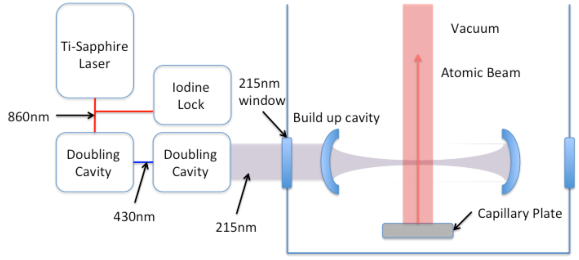
\includegraphics[width=6in]{ExperimentSetup.pdf}
\caption{\textcolor{blue}{should I use this because iodine lock versus rubidium lock}}
\label{ExperimentSetup}
\end{figure}

This thesis has both theoretical and experimental components. The experimental goals were to learn how to lock and operate the Ti:Sapphire laser. To excite krypton we needed to obtain $215$ nm light from the laser. However the parts needed to produce $215$ nm light were backordered. The Ti:Sapphire laser was also being used for a concurrent experiment designed to precisely measure the spectral lines of beryllium. For the beryllium experiment the Ti:Sapphire was used to produce $235$ nm light. All of the work done with the Ti:Sapphire laser in this thesis was done using the laser setup for the beryllium experiment and $235$ nm light. However, the process of producing and stabilizing the laser is exactly the same for the two projects. Future theses will design the optical cavity and couple the $215$nm light into the optical cavity, build the vacuum apparatus to house the optical cavity, and then optically produce metastable krypton atoms.

The theoretical portion of this thesis is to model the transfer of atoms from the ground state to the metastable state while passing through the light that is coupled to the optical cavity. The modeling was done three different ways, with each successive method involving a more complex, but more realistic condition.  


\section{Theory}

The outer electron shell of Krypton is completely filled because it is one of the noble gases; therefore the energy gap between the ground energy state and the first excited state is large. To laser cool from the ground state would require $123.5 nm$ light~\cite{FirstExcited} which is not currently experimentally possible using diode lasers. To be able to laser cool and trap krypton atoms they need to be in an excited state and that state needs to be metastable so that the atoms cannot decay during the cooling and trapping process. Krypton has a metastable state that is $~80,000 cm^{-1}$  $(\approx125 nm)$ above the ground state.  This metastable state, which is the lowest energy excited state, is doubly forbidden thus requiring three photons to transfer the atom from the ground state to the metastable state. In order to optically create metastable krypton atoms, we choose to excite the atoms into a higher energy excited state using a two-photon transition at $215 nm$. Once in this highly excited state, the atom can emit a photon (the third photon) and decay into the metastable state. 

To get the kryptons to the metastable state we used a $215 nm$ light to drive a two-photon transition from the ground $4p^6$ $^1S_0$ state, to the $5p_{[3/2]_2}$ state, see Figure~\ref{KrEnergyLevels}. Throughout our calculations we call the ground $4p^6$ $^1S_0$ state 'state 1' and the $5p_{[3/2]_2}$ state 'state 2.' There are other states at similar energies to the states in question, but they are not important for our experiment because the transitions are not resonant with our laser light, making it improbable for the atom to transfer to those states. From the $5p_{[3/2]_2}$ state the atom will either decay to an intermediate state and then ground state or it will decay to a metastable state, the $5s_{[3/2]_2}$ state. We called this metastable state 'state 3.' The last possibility is that the atom can ionize either from the the $5p_{[3/2]_2}$ state or the metastable $5s_{[3/2]_2}$ state. 

\begin{figure}[h!]
\centering
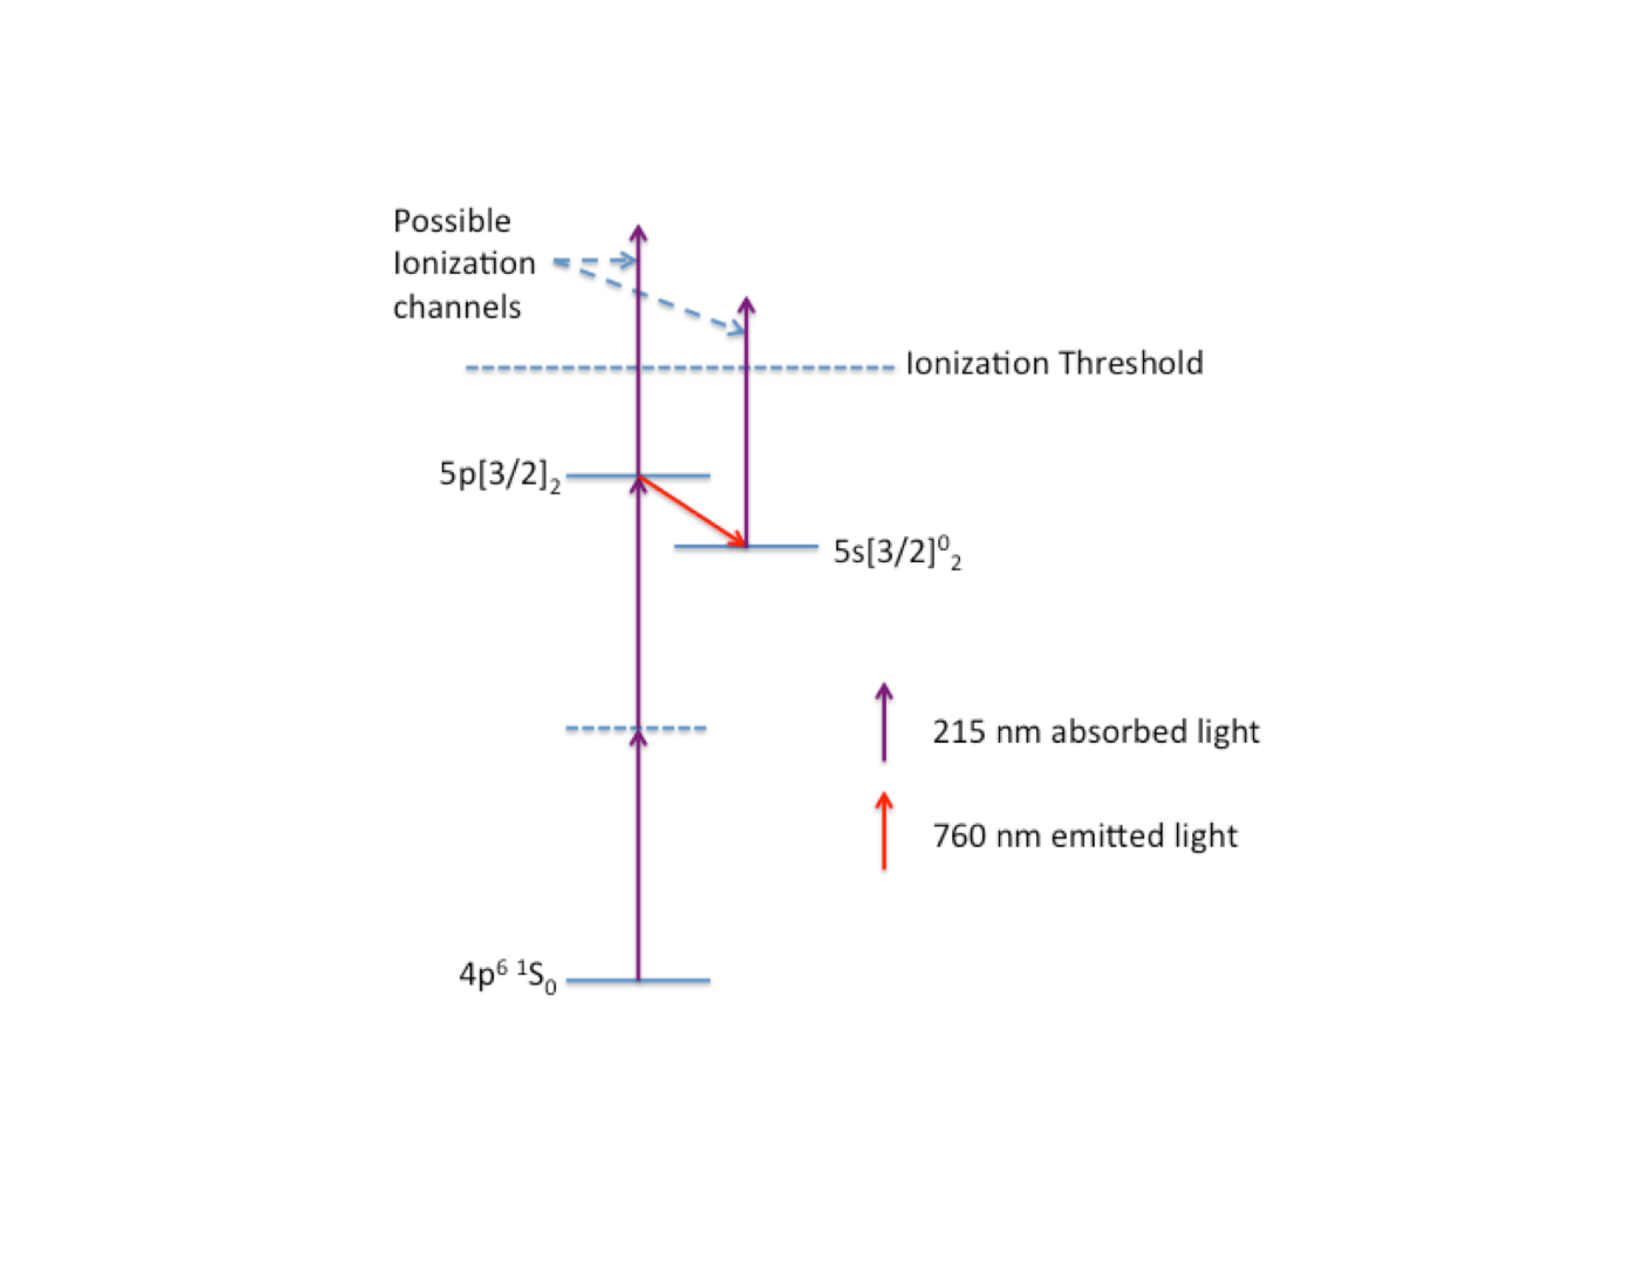
\includegraphics[width=4in]{KrEnergyLevels.pdf}
\caption{The energy levels of krypton. This figure only includes energy levels that are relevant to our experiment. Atoms are excited from the $4p^6$ $^1S_0$ state using two-photons to the $5p_{[3/2]_2}$ state then they decay either back to the $4p^6$ $^1S_0$ state or to the $5s_{[3/2]_2}$ state. Atoms can be ionized from both the $5s_{[3/2]_2}$ state and the $5p_{[3/2]_2}$ state.}
\label{KrEnergyLevels}
\end{figure}

Due to the isotope selectivity of laser cooling and trapping, Atom Trap Trace Analysis is able to count a specific isotope chosen by the laser frequency.  Only atoms in the metastable state can be trapped, so the efficiency of the apparatus is limited by the number of atoms transferred to the metastable state. To determine the efficiency of our set up, we calculated the percentage of krypton atoms that ended up in the metastable $5S_{[3/2]_2}$ state using the rate equations.

\begin{equation}
\label{RateEq1}
\frac{dN_1}{dt} = -\omega_{12}N_1 + \frac{1}{\tau_{21}}N_2
\end{equation}

Equation~\ref{RateEq1} gives the rate of change in the number of atoms ($N_1$) in the ground state. $\omega_{12}$ is the rate by which atoms in state 1 (the ground state) are excited to state 2, the $5P_{[3/2]_2}$ state, via the two-photon transition. The minus sign in front of $\omega_{12}$ indicates the atoms are leaving state 1. $\tau_{21}$ is the rate of decay from state 2 back to state 1. Similarly, there are differential equations for the three other states.

\begin{equation}
\label{RateEq2}
\frac{dN_2}{dt} = \omega_{12}N_1 -  \frac{1}{\tau_{21}}N_2 - \frac{1}{\tau_{23}}N_2 - R_2N_2
\end{equation}

\begin{equation}
\label{RateEq3}
\frac{dN_3}{dt} =  \frac{1}{\tau_{23}}N_2 - R_3N_3
\end{equation}

\begin{equation}
\label{RateEq4}
\frac{dN_4}{dt} = R_2N_2 + R_3N_3
\end{equation}

Where $\tau_{23}$ is the decay rate from state 2 to state 3, the metastable state. $\tau_{21}$ is the decay rate from state 2 to state 1, through an intermediary state. $R_2$ and $R_3$ are the ionization rates from states 2 and 3 respectively. $N_4$ is the number of atoms which have been ionized, just as $N_2$ and $N_3$ are the number of atoms in state 2 and state 3.

Solving these linearly dependent equations is possible, but the computational time is much shorter if they are put into matrix form.

\begin{equation}
\label{RateEqMatrix}
\begin{bmatrix}
	\frac{dN_1}{dt} \\
	\frac{dN_2}{dt} \\
	\frac{dN_3}{dt} \\
	\frac{dN_4}{dt} \\
\end{bmatrix}
=
\begin{pmatrix}
	-\omega_{12} & \frac{1}{\tau_{21}}  & 0 &  0   \\
	\omega_{12}  & -\frac{1}{\tau_{21}}- \frac{1}{\tau_{23}}-R_2 & 0 & 0 \\
	0  &  \frac{1}{\tau_{23}}  & - R_3 & 0 \\
	0  &  R_2  & R_3 & 0  \\
\end{pmatrix}
\begin{bmatrix}
	N_1 \\
	N_2 \\
	N_3 \\
	N_4 \\
\end{bmatrix}
\end{equation}

The general solution to the first order differential matrix equation is
\begin{equation}
\label{RateEqSol}
N(t) = A_1e^{\lambda_1 t} v_1 + A_2e^{\lambda_2 t} v_2 + A_3e^{\lambda_3 t} v_3 + A_4e^{\lambda_4 t} v_4 
\end{equation}

where $\lambda$ is an eigenvalue of the matrix and $v$ is an eigenvector of the matrix. $A$ is the amplitude determined by the initial conditions. The our initial condition is that all of the atoms are in the ground state, state 1. That is
\begin{equation}
\label{InitialCond}
N_1(0) = 1, \	\	\	\	
N_2(0) = 0, \	\	\	\	
N_3(0) = 0, \	\	\	\	
N_4(0) = 0 
\end{equation}

which allows us to obtain particular solutions to the rate equations. We did all calculations and analysis in Mathematica. Once we had the solutions to the rate equations we needed to define the variables $\omega_{12}$, $\tau_{21}$, $\tau_{23}$, $R_2$ and $R_3$ which make up the eigenvectors and eigenvalues of the matrix.

\subsection{Constant Intensity and Velocity Approximation} 

For our initial calculation we made a couple simplifying approximations. The first approximation we made was to model the intensity of the laser beam profile a step function.  Although the actual laser beam has a gaussian profile, this approximation allows for an exact solution to the above equations.  The height of the step function was constant and set equal to the maximum of the gaussian profile intensity. The width was set to twice the laser waist (also known as the laser radius) of the gaussian laser beam profile.  The second approximation was to assume all of the atoms in the collimated atomic beam were traveling with the root-mean-squared velocity of the atomic beam's Maxwell velocity distribution.  These two approximations are standard in the community for evaluating the rate equations.  We later expanded our calculations to account for the gaussian beam profile and the velocity distribution; those calculations can be found in the subsequent sections. 

The decay rates for state 2 ($5P_{[3/2]_2}$) to state 1 (ground state) and state 3 (metastable state) are know quantities.~\cite{KrTransitions}
\begin{equation}
\label{DecayRates} 
\tau_{21} = 1.1x10^7 s, \	\	\	\	 \tau_{23} = 3.1x10^7s
\end{equation} 

The ionization rates are given by 
\begin{equation}
\label{IonizationRates}
R = \sigma_{pi} \frac{I}{\hbar\omega}
\end{equation}

where $I$ is the intensity of the laser calculated from power, $I = \frac{P}{\frac{1}{2}\pi w^2}$ and $w$ is the beam waist. We used a power value of $7.5 W$ based on a conservative estimate from the laser specifications. $\omega$ is the angular frequency of the light defined as $\omega = \frac{2\pi c}{\lambda}$. $\sigma_{pi}$ is the photo-ionization cross section, which contributes to the rate by which photons will be absorbed by the atom. $\sigma_{pi2} = .5$ Mbarn for the $5p_{[3/2]_2}$ state and $\sigma_{pi2} = .25$ Mbarn for the $5s_{[3/2]_2}$ state.~\cite{Cannon} 

The rate by which atoms are excited by two-photon transition from state 1 to state 2 is $\omega_{12}$ given by
\begin{equation}
\label{ExcitationRate}
\omega_{12} = \sigma_0\ g\ \frac{I^2}{(\hbar \omega)^2}
\end{equation}

$\sigma_0$ is the two-photon cross section, the probability that two photons will be absorbed, which is $4.4x10^{-35} cm.^{-4}$~\cite{NIST} $g$ is the on resonance line shape factor, defined as 

\begin{equation}
\label{LineShapeFactor}
g = 2 \sqrt{\frac{Log(2)}{2 \pi (\Delta \omega_L^2 + \Delta \omega_D^2)}}
\end{equation}

with $\Delta\omega_L$ as the line width of the laser. $\Delta \omega_D$ is Doppler line width for the two-photon transition, which is zero in our case because the krypton atoms are moving perpendicular to the laser.  The line shape factor becomes important whenever the line width of the transition is smaller than the line width of the laser.  When this happens, different frequencies of the light have different probabilities of exciting the atom.  The line shape factor, which is a convolution between the gaussian line shape of the laser and the Lorentzian line shape of the atomic transition, takes into account the varying transition probability across the frequency profile of the laser beam. 

The solution to these equations for $7.5 W$ of power inside the build up cavity is given in Figure~\ref{MetaGraph1} which shows the fraction of atoms in the metastable state as a function of the size of the laser's beam waist. The optimum number of atoms end up in the metastable state when the beam waist is close to 20 microns. When the beam waist is smaller than 20 microns more of the atoms are ionized since the intensity is large. When the beam waist is larger than 20 microns, the intensity is too small to drive the two-photon transition leaving most of the atoms in the ground state.

\begin{figure}[h!]
\centering
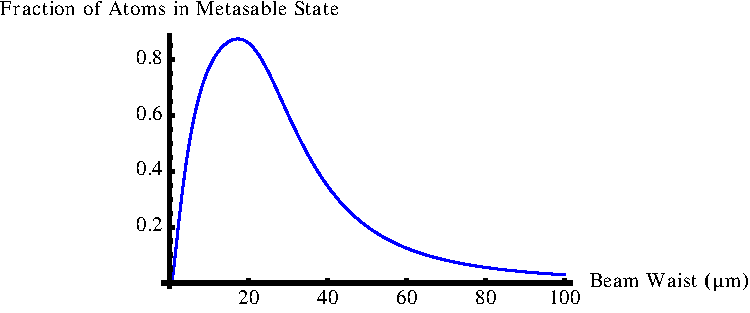
\includegraphics[width=6in]{MetaGraph1.pdf}
\caption{The fraction of atoms in the metastable state as a function of laser's beam waist. The fraction of atoms reaching the metastable state increases sharply as the beam waist increases until 20 microns. After 20 microns the number of atoms in the metastable state decreases because the intensity is too small.}
\label{MetaGraph1}
\end{figure}

Figure~\ref{TimeGraph} shows the fraction of atoms in each of the states as a function of time for a laser waist of $20 \mu m$, which is helpful to see how the atoms move between states. The green line is the ground state which starts at one, because the initial condition is that all of the atoms are in the ground state, and continuously decreases as time passes. State 2 is the orange line; it quickly increases as atoms are excited through two-photon transition. The number of atoms in state 2 decreases as atoms decay either back to the ground state or to the metastable state. The number of atoms in the metastable state increases as atoms decay to it from the state 2. Atoms only leave the metastable state if they ionize. For this laser waist, only a small fraction of atoms are ionized, see the red line.  The final number of atoms in the metastable state given in Figure~\ref{MetaGraph1} is the number of atoms in state 3 at the end of the atom-light interaction time (the last point on the plot in Figure~\ref{TimeGraph}) plus the fraction of atoms in state 2 that will naturally decay to state 3, about 74 percent. which means that the fraction of atoms reaching the metastable state is constant through time.

\begin{figure}[h!]
\centering
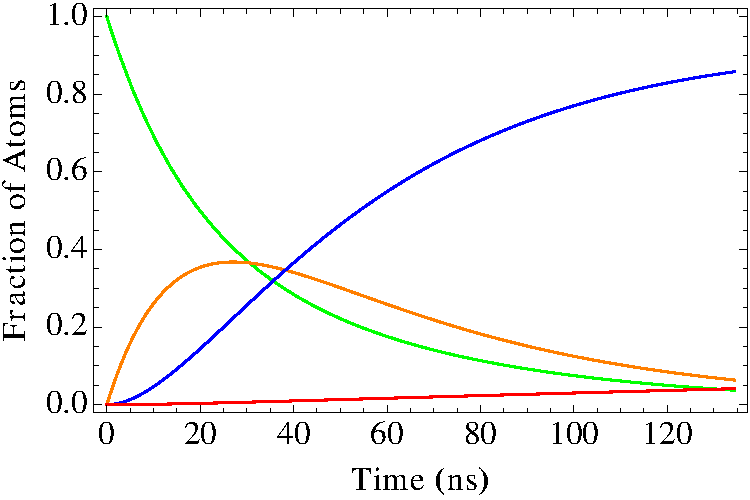
\includegraphics[width=6in]{TimeGraph.pdf}
\caption{The fraction of atoms in each state plotted against time. The green line is the ground state. The orange line is the excited $5p_{[3/2]_2}$ state. Blue is the metastable $5s_{[3/2]_2}$ and red is the fraction of atoms that have ionized.}
\label{TimeGraph}
\end{figure}

\subsection{Gaussian Beam Profile}

To make our model more accurate we factored in the intensity profile of the laser beam. From the laser manufacturer's, M Squared, specifications we know that the Ti:Sapphire laser's intensity profile is a two-dimensional gaussian. It was conceptually simple to incorporate the intensity profile into our previous calculation in place of the constant intensity. Computationally, it was not quite as easy.

We replaced our former intensity with $I = I_0 e^{\frac{-2 x^2}{w^2}}$ where $I_0 = \frac{P}{\frac{1}{2}\pi w^2}$, the same intensity we used as a constant in our previous approximation. However, the addition of the gaussian term means that the equations no longer have analytical solutions and instead required us to solve them numerically.

The resulting graph is noticeably different from our first approximation, see Figure~\ref{AllGraph}. Adding the intensity profile does not change the shape of the peak, but it does make the peak lower and shifts it to the right. The location of the peak is now around 15 micrometers, rather than the 20 micrometers from the constant intensity approximation.  The fraction of atoms reaching the metastable state is still quite high having been decreased by just over five percent from roughly .9 to .85.

\begin{figure}[h!]
\centering
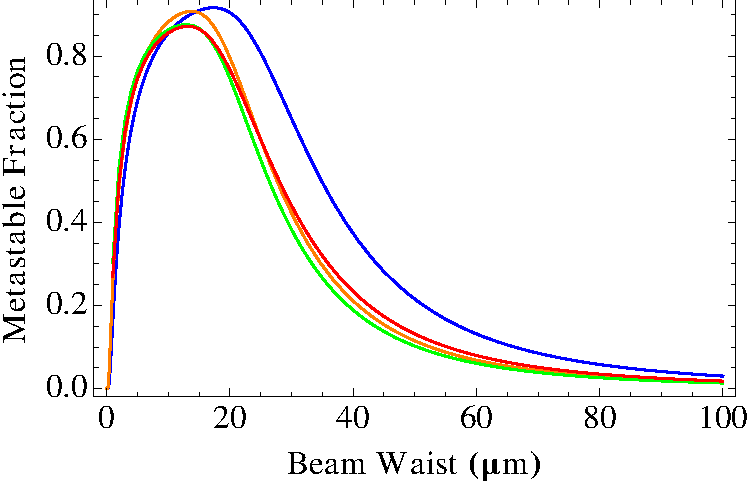
\includegraphics[width=6in]{AllGraph.pdf}
\caption{The blue line represents the calculation assuming all atoms have the same velocity (the root-mean-square velocity) and a constant intensity. The green line represents the calculation assuming the root-mean-square velocity and a gaussian intensity profile. Finally, the red line is the calculation using both the gaussian intensity profile and the Maxwell velocity distribution. The root-mean-square velocity is a good approximation; the green and red lines are very close. The constant intensity is not as good an approximation for the more accurate gaussian intensity profile, note the differences between blue line and the green line.}
\label{AllGraph}
\end{figure}


\subsection{Maxwell Velocity Distribution}

Adding the Maxwell velocity distribution presents new difficulties. To account for the range of velocities we first calculated the fraction of atoms in each of a series of velocity intervals. Then we calculated the fraction of atoms from each interval, that is from each different velocity range, that reach the metastable state. We then multiplied the fraction of atoms that reach the metastable state from a velocity interval by the fraction of atoms in that velocity interval. Then we added together the resulting fraction from each interval to obtain the total fraction of atoms that end up in the metastable state.  In other words, we evaluated the probability an atom gets transferred to the metastable state for all velocities and then weighted those probabilities according to the Maxwell velocity distribution.  See Figure~\ref{AllGraph} for a comparison of the fraction of atoms reaching the metastable state from each calculation.

Modeling the velocity of the atoms as the root-mean-square velocity is a very good approximation. The differences between using the root-mean-square velocity as a single average value and using the Maxwell velocity distribution were quite small. See the similarity between the green and red lines in Figure~\ref{AllGraph}.  This result gives us confidence that in future calculations we do not have to use the computation time to take into account the full Maxwell distribution.
  

\section{Titanium-Sapphire Laser}

A titanium-sapphire (Ti:S) laser uses titanium doped sapphire crystal as the lazing medium, hence the name. Ti:Sapphire crystals are made by doping $\text{Al}_2\text{O}_3$ with $\text{Ti}^{3+}$ ions which replace some of the $\text{Al}^{3+}$ ions.~\cite{Ti:S} The crystal is placed inside a ring optical cavity, see Figure~\ref{InsideTiS}. Ti:S crystals are used because they have a broad range for absorption and emission of light. They can absorb light ranging from $\approx 400 nm$ to $\approx 600 nm$ and emit light from $\approx 700 nm$ to $\approx 1000 nm$.~\cite{Ti:S} Because the Ti:S emits so many wavelengths, to obtain monochromatic light the range of wavelengths is narrowed using a birefringent filter. Various wavelengths experience different transmission rates through the birefringent filter, because the refractive index of the filter changes the effective length of the resonance cavity causing some wavelengths to de-constructively interfere. Rotating the birefringent filter selects roughly for the desired wavelength. The birefringent filter is a rough selection, the band of wavelengths is still large (around 20 GHz). To further narrow the bandwidth the Ti:S uses an etalon. The etalon is a crystal which also changes the effective resonance length of the cavity. By tuning the angle of the birefringent filter and etalon together, a single frequency mode with a width of about 5 MHz can dominate the resonance structure of the cavity. The each previously emitted photon passing through the Ti:Sapphire crystal again emits two photons, exponential growth. Due to this exponential growth inside a lazing medium, the resonant laser mode dominates all other modes. The optical diode in Figure~\ref{InsideTiS} is an optical element that stops the laser light from traveling the wrong direction in the cavity.  The crystal itself is pumped using a Coherent Verdi-V18, which is a diode-pumped laser emitting green $(532nm)$ light. The pump laser could be operated at various powers which adjusted the overall output of the Ti:Sapphire laser. We operated the pump laser at both 18 W and 12 W.

All the optical components in the SolsTi:S from M Squared are automated. The desired wavelength is selected on the laptop and the birefringent filter and etalon adjust automatically.

\begin{figure}[h!]
\centering
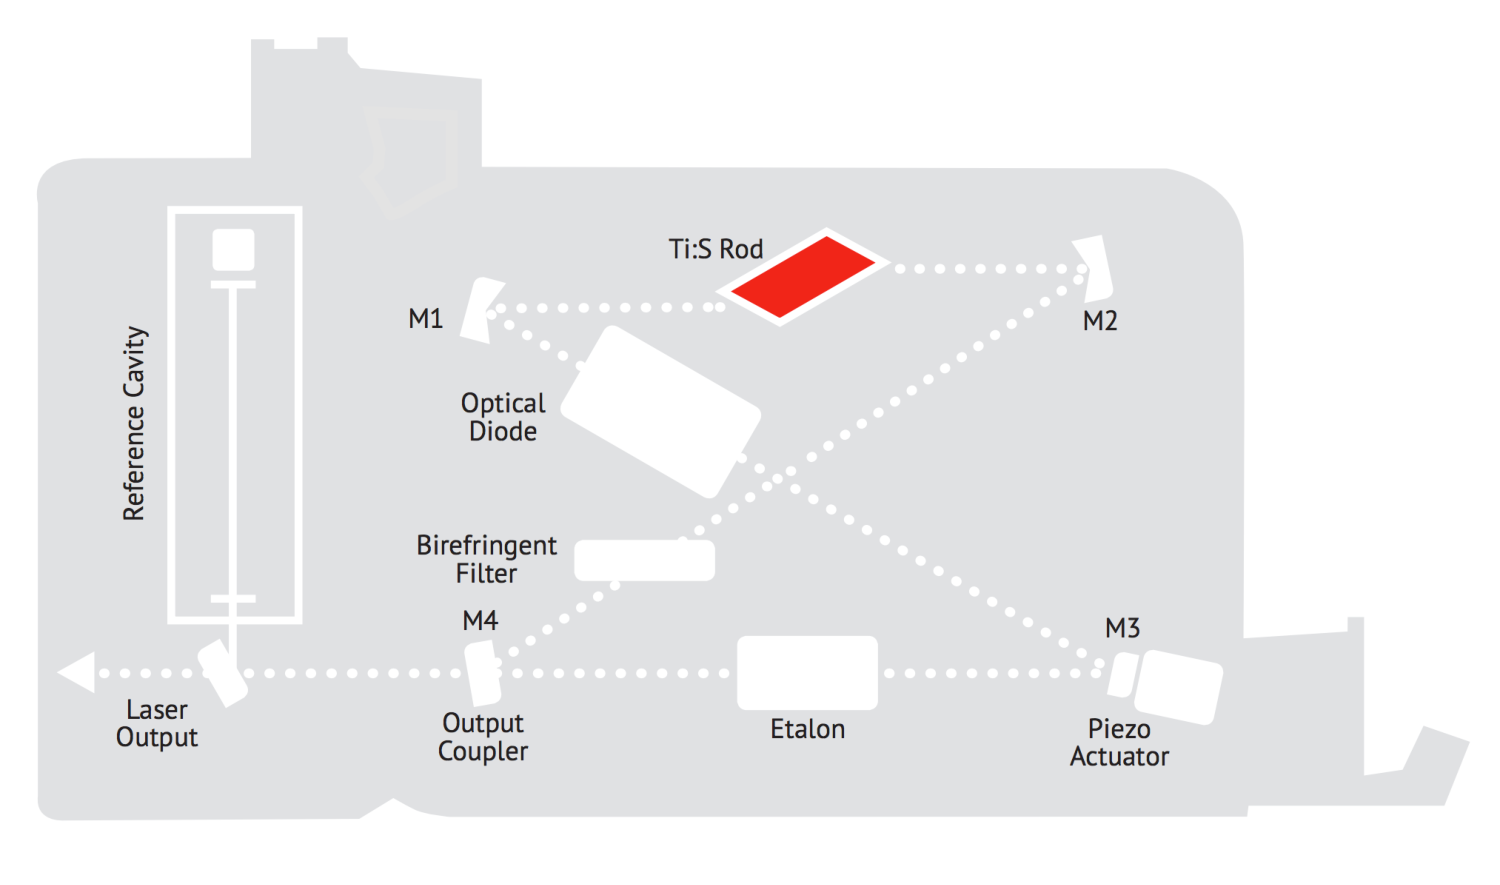
\includegraphics[width=6in]{InsideTiS.pdf}
\caption{The optical setup of the Ti:Sapphire laser. Light from the pump laser is coupled into the Ti:Sapphire at M2. The red trapezoid is the Ti:Sapphire crystal. The birefringent filter and the etalon both change the length of the optical cavity as does the piezo actuator attached to M3. The optical diode prevents the light from traveling the opposite direction in the cavity. After the Ti:Sapphire cavity the light is locked to the reference cavity before leaving the laser.~\cite{Ti:S}}
\label{InsideTiS}
\end{figure}

The laser light exits the ring cavity through the output coupler. This single mode light is then sent to the reference cavity. The reference cavity is a confocal Fabry-Perot cavity.  Since there are no optical elements in this cavity, wavelengths that fit in integer multiples into resonator length constructively interfere and all other wavelengths interfere de-constructively. In the confocal configuration, the resonant condition is $L=n \lambda/4$ where $n$ is an integer. The purpose of this cavity is to further reduce the frequency width of the laser. Once the etalon is locked to a particular lazing mode, which is discussed below, the laser can be stabilized to the reference cavity. The resonance width of the reference cavity is less than 50kHz. Once locked to the reference cavity, that signal can be fed back to the etalon. This feedback signal can be used to correct the angle of the etalon further narrowing the frequency width of the laser to, at best, the resonance width of the reference cavity. After stabilization to the reference cavity, the frequency width of the Ti:S laser is approximately 50 kHz.

Once both the etalon and reference cavity signals are stabilized, both the angle of the etalon and the length of the reference cavity can be changed simultaneously.  Moving the two optical elements together adjusts the wavelength of the laser such that it is still resonant with both the ring optical cavity and the reference cavity.  This is how the Ti:S laser frequency is scanned in a controlled manner. The scan range of this laser is approximately 25 GHz, limited by the distance to the neighboring resonance mode.  

Other important laser parameters include amplitude noise, the spatial mode, the beam radius, and the beam divergence.  From the data sheet, the amplitude noise is less than $0.1\%$ RMS above the Verdi pump laser.  The output mode is the lowest energy spatial (Gaussian) mode, also known as the ${TEM}_{00}$ mode.  The beam radius is about $0.4 mm$ with a divergence of less than $1.5$ mrad.  Finally the output polarization is horizontal.

After the laser light leaves the Ti:S laser and reference cavity, it then consecutively passes through two frequency doubling cavities. Refer to Figure~\ref{LaserSetup} for the experimental set-up of the laser. Each doubling cavity is preceded by a beam splitter module and an alignment module. The beam splitter module allows us to "pick-off" a portion of the laser light to use in another experiment or to monitor the laser. The alignment module contains a mirror that allows us to spatially align the laser with the doubling cavity. There is also a beam splitter module and beam alignment module between the pump laser and Ti:S laser. This beam splitter module will be used in the beryllium experiment in a separate mixing cavity to produce 332nm light. The alignment module is to optimize coupling into the Ti:S laser.

\begin{figure}[h!]
\centering
\includegraphics[width=6in]{LaserSetup.pdf}
\caption{The experimental set-up of the Ti:S laser comprised of a pump laser, Ti:S laser, reference cavity, doubler and quadrupler. Each component is separated by a beam splitter and a beam aligner, which consists of a set of mirror to adjust the beam along each axis.}
\label{LaserSetup}
\end{figure}

The doubling cavities behave very similarly to the ring cavity inside the Ti:S laser. Instead of a titanium doped sapphire crystal, a strongly birefringent nonlinear crystal is used. These crystals are capable of absorbing two photons and emitting a single photon with twice the energy. As a result, the wavelength of light is cut in half while the frequency doubles. Sending the light through the crystal once will convert some of the $860$ nm light into $430$ nm light. However typically a nonlinear crystal has a very low efficiency $(\approx .01\%)$.~\cite{ECDX} Placing the crystal in the cavity allows many more opportunities for the light to be converted. Also, since the crystal is nonlinear, the cavity provides a much higher intensity further increasing the efficiency of the doubling medium. A standard Barium borate (BBO) crystal check this is used in the first frequency doubling cavity to convert $860$ nm light to $430$ nm light for the krypton project or to convert $940$ nm light to $470$ nm light for the beryllium project. The second doubling crystal is very similar to the first, but uses a crystal \textcolor{blue}{what type of crystal is this?} designed to double $430$ nm light to $215$ nm light for the krypton project or \textcolor{blue}{add crystal type} to double $470$ nm light to $235$ nm light for the beryllium project.

\section{Operating Procedure}

The first step to operating the laser is to turn on the water coolers which cool the sapphire crystals and the pump laser and then to turn on the pump laser and allow it to warm up and stabilize. The pump laser takes around thirty minutes to warm up, before it is warm it will not generate any light from the Verdi laser. It is preferable to allow the pump laser longer to fully stabilize because any drift in the pump laser will cause the Ti:Sapphire deviate from optimum and likely lose lock. When locking the laser we are stabilizing the frequency of the light to the resonance length of a cavity. After the pump laser is warm and stable, the shutter should be opened allowing light to pass into the Ti:Sapphire laser. The light from pump laser heats up the Ti:Sapphire crystal while the water coolers cool it down. The Ti:Sapphire crystal should be given ten to fifteen minutes to reach thermal equilibrium before locking is attempted.  

Once the Ti:Sapphire crystal's temperature is stabilized, the light from the pump laser into the Ti:Sapphire laser must be optimized. As mentioned in the previous section, the output from the pump laser first passes through a beam splitter module and then an alignment module. The alignment module can be used to adjust the beam in the horizontal and vertical directions to optimize the coupling into the Ti:Sapphire laser ring cavity. The power to the Ti:Sapphire laser can be measured by using the beam splitter module after the Ti:Sapphire laser and reference cavity, again see Figure~\ref{LaserSetup} and a power meter. The alignment in the $z$ direction, the direction of propagation, should not be adjusted using the alignment module. To change the location of the beam waist, the $z$ alignment of the beam, a lens should be used after the beam leaves the Ti:Sapphire set-up. The horizontal and vertical directions, $x$ and $y$, should both be adjusted to maximize the output power of the Ti:Sapphire laser. 

The alignment of the birefringent filter and etalon in the Ti:Sapphire laser are controlled from a laptop using the provided software. The desired wavelength is selected on the laptop. After selecting the wavelength, the first step is "lock" the etalon to the desired angle.To do this, we first need to produce an error signal that can be used as a feedback mechanism. The etalon error signal (Figure~\ref{EtalonError}) is the power generated as the resonance length of the ring cavity. The signal peaks when the etalon and birefringent filter align such that a resonant mode is at the frequency of maximum transmission through the birefringent filter. The dips occur when the resonant mode no longer lines up with maximum transmission of the birefringent filter and the following peak is when the next resonant mode is in alignment. In short, the etalon error signal is nothing more than the power fluctuations that result from scanning over etalon modes. 

To mechanically scan across etalon modes, the length of the ring is changed by a piezo electric transducer (PZT) which is attached one of the mirrors. When a voltage is applied to the PZT, the length of the transducer changes. This PZT operates between 0 and 200 V. To create the error signal, this PZT is check the number dithered at around 19 kHz with an amplitude suitable to include more than one resonant mode. It should be emphasized that at the moment the laser bandwidth is determined by the birefringent filter. The etalon is locked at a point where its error signal crosses zero. Refer to Figure~\ref{EtalonError}. The idea is that if the voltage is positive, the resonance length of the ring cavity will be slightly adjusted in one direction so the voltage returns to zero.  If the voltage is negative, the resonance length is slightly adjusted in the opposite direction keeping the error signal voltage at zero. The etalon error signal can be seen by selecting 'Etalon Error' from the dropdown menu for one of the monitors and scanning the resonator cavity continuously. The etalon error signal can be seen on the oscilloscope; if it is not symmetric around zero, the pump laser may need to be re-optimized into the Ti:Sapphire laser using the alignment module.  The etalon is then locked by clicking 'Apply Lock' on the computer. The locked signal should be a zero and show only noise. The signal to noise ratio for the etalon is 13. When locked, the PZT voltage should be close to $100 V$, if the voltage on the PZT is not within $100 \pm 15 V$ the laser is not locked even if the software reports otherwise. After the etalon is locked, the frequency width of the laser is reduced from $~20$ GHz (the line width of the birefringent filter) to $~5$ MHz.

\begin{figure}[h!]
\centering
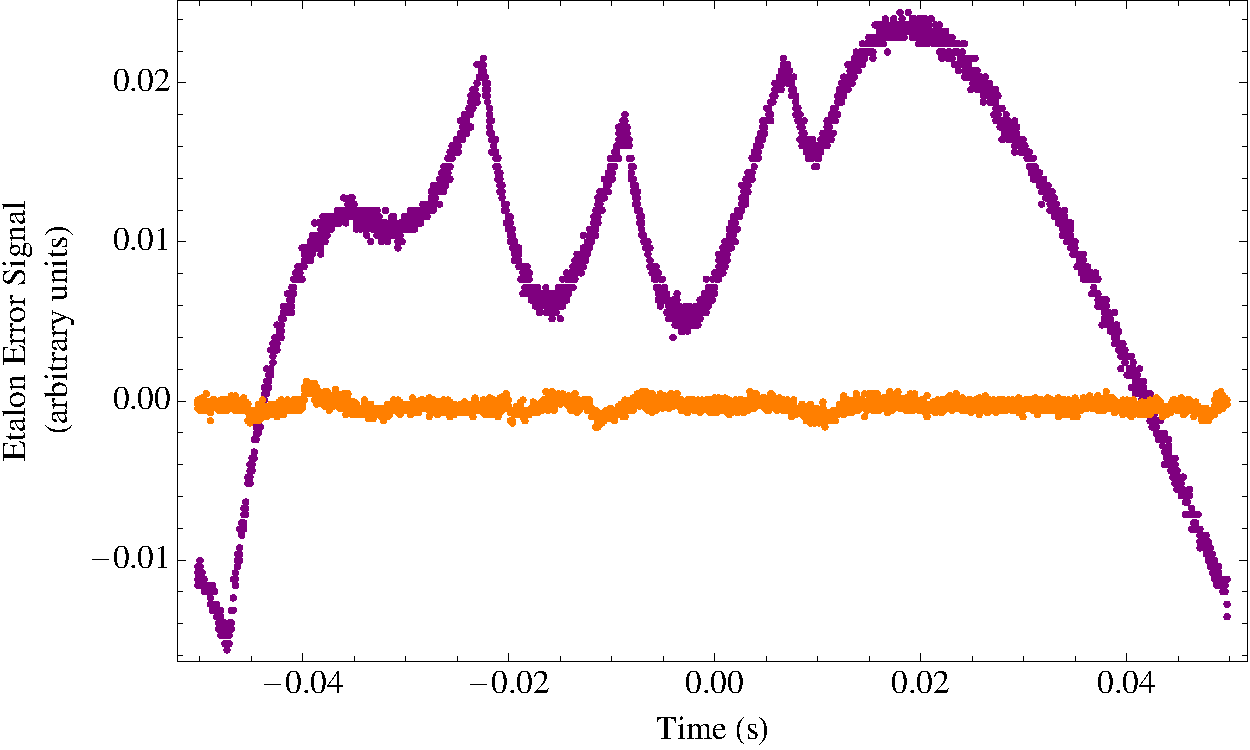
\includegraphics[width=6in]{EtalonError.pdf}
\caption{The etalon error signal as seen on the oscilloscope both before, maroon, and after, orange, the etalon has been locked. The unlocked error signal is the changes in power as the resonance length of the cavity is scanned. The peaks are when the resonant mode of the etalon matches the maximum transmission through the birefringent filter and the dips and when the resonant mode and maximum transmission are not aligned. The signal to noise ratio is 13.}
\label{EtalonError}
\end{figure}

The second step of locking the Ti:Sapphire involves stabilizing the etalon locked output to the reference cavity. The reference cavity further narrows the bandwidth of the laser.  The reference cavity signal feeds back to the PZT controlling the ring cavity resonance length. When stabilized, the laser frequency is "locked" to the length of the reference cavity. If the cavity length drifts, so does the voltage of the PZT and thus the frequency of the laser. The bandwidth of the reference cavity is much smaller than the bandwidth of the etalon. Therefore this feedback is constantly correcting the length of the cavity and thus the laser frequency. The result is the bandwidth of the reference cavity is mapped back on to the etalon producing laser light whose laser bandwidth is just slightly larger than that of the reference cavity.

To view the reference cavity error signal, the reference cavity length is scanned. The length of the reference cavity is controlled by a second PZT with the same properties as the PZT controlling the ring cavity length. When the length of the cavity matches the resonant condition, $L=n \lambda/4$, light is transmitted through the cavity and detected by a photodetector. The program is used to scan the reference cavity continuously and selecting "reference error" from the monitor menu outputs the error signal to the oscilloscope. The reference cavity error signal is created by subtracting the photodetector signal from a reference voltage, see Figure~\ref{ResonatorError}. The DC offset is added because the reference error must cross zero to support a good lock, if the reference error does not cross zero it should be adjusted by clicking on the "PD Trim" button and a raising or lowering the "Ref Cavity PD Gain" in the pop-up window. This type of lock is referred to as a side lock. The error signal is fed back to the reference cavity PZT. If the error signal becomes positive or negative the PZT shortens or lengthens the cavity so the error signal returns to zero.

Once locked the reference error should be zero on the oscilloscope and the reference cavity PZT should read $100 \pm 15 V$ on the laptop. As can be seen in Figure~\ref{ResonatorError}, the signal error ratio for the reference cavity is large, 377. If the error signal has features in between the typical cavity modes, which would show up as small peaks between the large peaks or large peaks that are unevenly spaced in Figure~\ref{ResonatorError},  the Ti:S laser is not running in a single longitudinal mode. To correct this, the etalon should be unlocked and the coupling of the pump laser should be re-optimized. This is most likely to happen if the laser is not fully warmed up before locking the etalon.

\begin{figure}[h!]
\centering
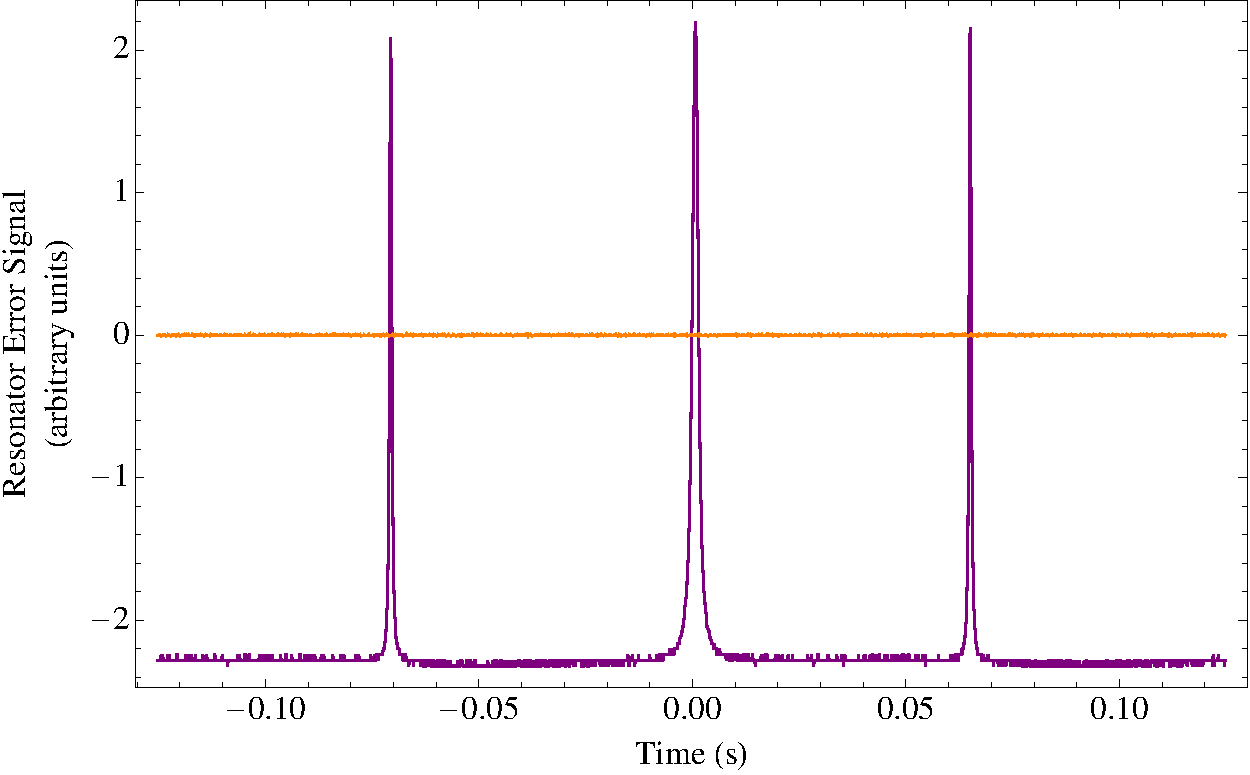
\includegraphics[width=6in]{ResonatorError.pdf}
\caption{The maroon line is the reference cavity error signal before it is locked and the orange line is after the resonator has been locked. The cavity will be locked to one side of the peak. A sharp peak means that small changes in the power result in large changes in the error signal and cause the PZT to adjust the cavity length. The signal to noise ratio is 377.}
\label{ResonatorError}
\end{figure}

Next the laser light must be coupled from the Ti:Sapphire laser into the ECD-X, Ultra-compact Frequency Doubling Accessory. The light passes through another beam splitter module and then through an alignment module to couple the Ti:Sapphire light into the EDC-X, refer back to Figure~\ref{LaserSetup}. The beam splitter module is to be used to stabilize the laser to an atomic or cavity reference. Stabilizing the laser frequency to a  rubidium cell is covered in the next section.

To optimize the light into the ECD-X, look at ``ECD PD 1'' on the oscilloscope and adjust the mirrors in the horizontal and vertical directions between the reference cavity and the ECD-X. The voltage of the ECD photodiodes (PD 1 and PD 2) should be optimized at the same mirror alignment, by maximizing the voltage on the oscilloscope. After maximizing PD 1, confirm the alignment by checking that PD 2 is also maximized.

Experience has shown that ECD-X, the doubler, is the most difficult to lock. It is extremely sensitive to instability in the etalon error and reference cavity error; if they are locked more than $8$ V away from $100$ V the ECD-X is unlikely to lock. 

Next the error signal can be examined on the oscilloscope. The ECD error signal is created using the H�nsch-Couillaud technique. The laser light enters the cavity and passes through the birefringent crystal. Due to differences in finesses, the birefringent crystal has different transmission rates different directions of polarization. These different losses cause the two polarizations to be out of phase when the frequency of the light does not match the resonance condition of the cavity. The difference in phase is detected by passing the light trough a quarter wave plate then a linear polarizing beam splitter. The intensities of both polarizations are detected by photodiodes. The subtraction of the two photodiode signals is the error signal that is fed back to a PZT that controls the cavity length.

To see the error signal on the oscilloscope select ``ECD error'' from the monitor menu and start a continuous scan of the ECD. An example of the ECD error, before and after it is locked, is in Figure~\ref{ECDError}. If the ECD does not cross zero, open the ECD adjustment window on the laptop by clicking ``ECD'' then adjust ``PD 1 gain'' and ``PD 2 gain'' until the ECD error signal crosses zero. The ECD usually requires a slight offset from zero to lock. If the ECD does not lock when the lock is applied, increase the ``Aux PD gain'' (also in the ECD window.) If the ECD is still not locking, the reference cavity and etalon should be unlocked, re-optimized and relocked. The ECD has a signal-to-noise ratio of 27.

\begin{figure}[h!]
\centering
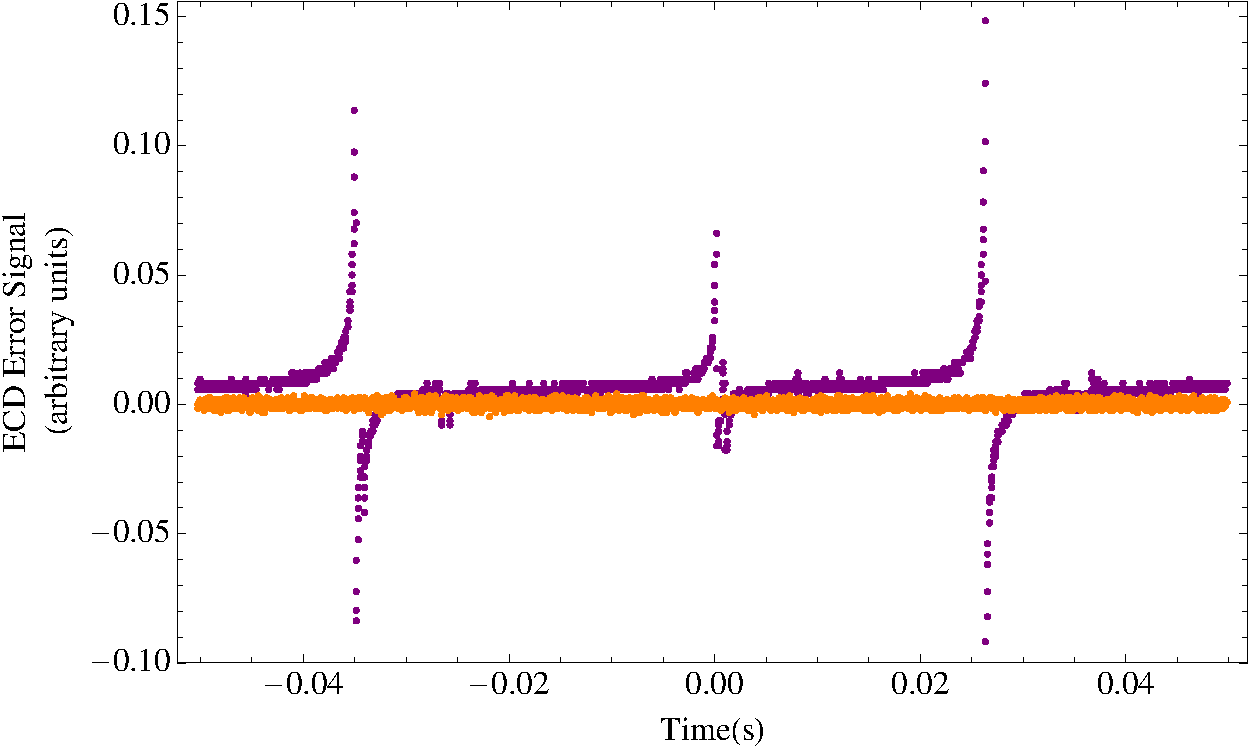
\includegraphics[width=6in]{ECDError.pdf}
\caption{The maroon line is the ECD error signal before it is locked, which is difference between PD 1 and PD 2. After it has been locked, the error signal is the orange line. The signal to noise ratio is 27.}
\label{ECDError}
\end{figure}

Once the doubler (ECD-X) has been locked the final step is locking the quadrupler (ECD-X-Q.) The process of locking the quadrupler is similar to the process of locking the doubler. The software required to control the quadrupler is a different package from the other sections of the laser, switch to the other control console on the laptop. Just like the doubler, the quadrupler is optimized by looking at PD 1 and PD 2 on the oscilloscope. They should be optimized by adjusting the beam alignment in the horizontal and vertical directions. The error signal is produced using the H�nsch-Couillaud technique, see above. The ECD-X-Q error can been seen on the oscilloscope and adjusted in the same manner as the ECD-X. It most cases the quadrupler will lock with more ease than the doubler. The locked and unlocked error signals can been seen in Figure~\ref{ECDQError}. The signal-to-noise ratio is 9.

\begin{figure}[h!]
\centering
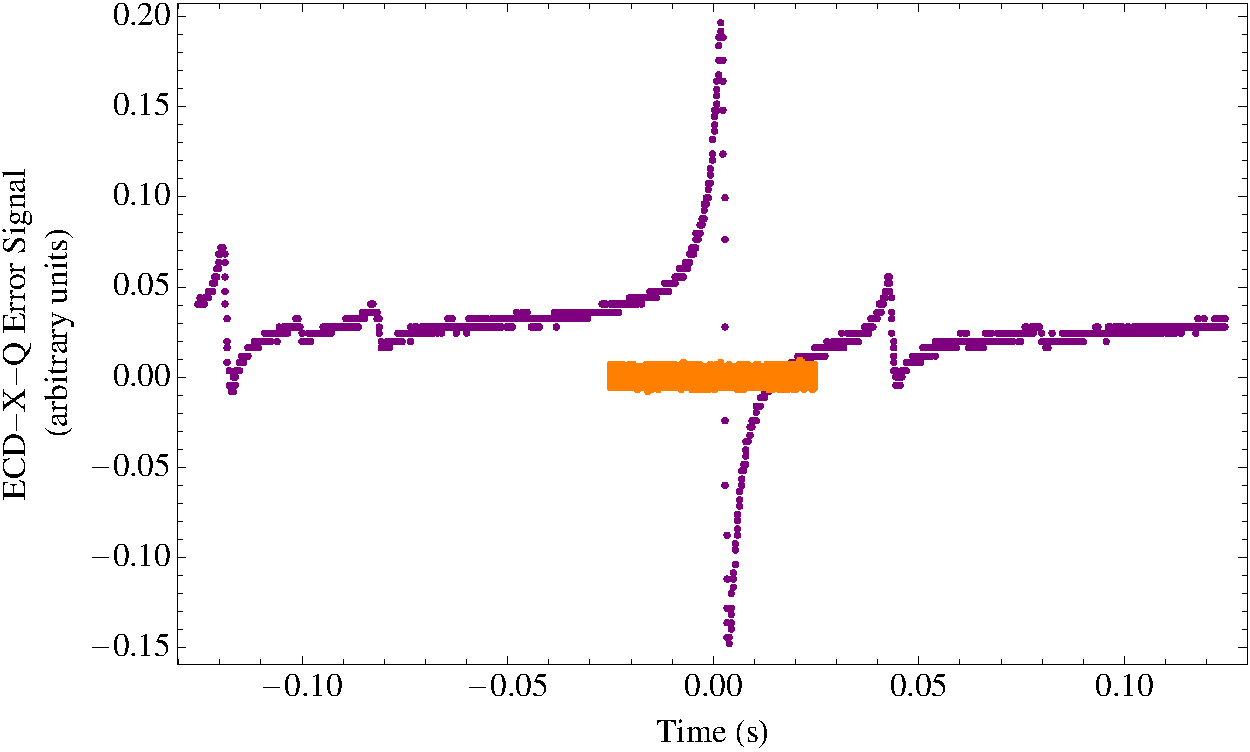
\includegraphics[width=6in]{ECDQError.pdf}
\caption{The maroon line is the ECD-X-Q error signal before it is locked, which is difference between PD 1 and PD 2. After it has been locked, the error signal is the orange line. The signal to noise ratio is 9.}
\label{ECDQError}
\end{figure}

The quadrupler lock is sensitive to vibration and likely to unlock. The reference cavity is more stable, but can also unlock particularly if the pump laser drifts. The lock voltages should be checked periodically while working with the laser to ensure that lock has not been lost. If the lock voltages on the laptop have a difference greater than $15 V$ from $100 V$ than lock has been lost even if the laptop does not read ``lock error.'' When the lock fails the laser should be unlocked and relocked, with re-optimization if necessary.

When turning off the laser all locks should be removed. Then the pump laser shutter should be closed, blocking all light into the Ti:Sapphire laser. Afterwards the pump laser can been cooled if the setup will not be used for an extended period.

\section{Absolute Stabilization}

Locking the Ti:Sapphire laser stabilizes the internal components of the laser to each other and keeps the laser operating on a single spacial mode. However, all of the components of the Ti:Sapphire are susceptible drift due to thermal or vibrational effects which can adjust the length of the resonance lengths of the Ti:Sapphire, the reference cavity, the doubler, and the quadrupler. Both the experiments using the Ti:Sapphire laser require precise, stable frequencies. Producing metastable krypton atoms using the Ti:Sapphire requires $215$ nm light whose wavelength does not fluctuate. Preforming precise beryllium spectroscopy necessitates knowing the frequency of the laser very accurately. All of which means that Ti:Sapphire laser needs to be externally stabilized to a reference that will not fluctuate or drift.

In the future, we will most likely stabilize the Ti:Sapphire laser to an iodine lock or an ultra low expansion (ULE) optical cavity. Currently we are planning to stabilize to a cesium or rubidium transition using sub-Doppler spectroscopy. The optical setup can be seen in Figure~\ref{SubDoppler}. Sub-Doppler spectroscopy is a rather ingenious application of the Doppler shift and multiple laser beams to produces a sharp, precise peak which can then be used for an on resonance, top-of-fringe, lock.

\begin{figure}[h!]
\centering
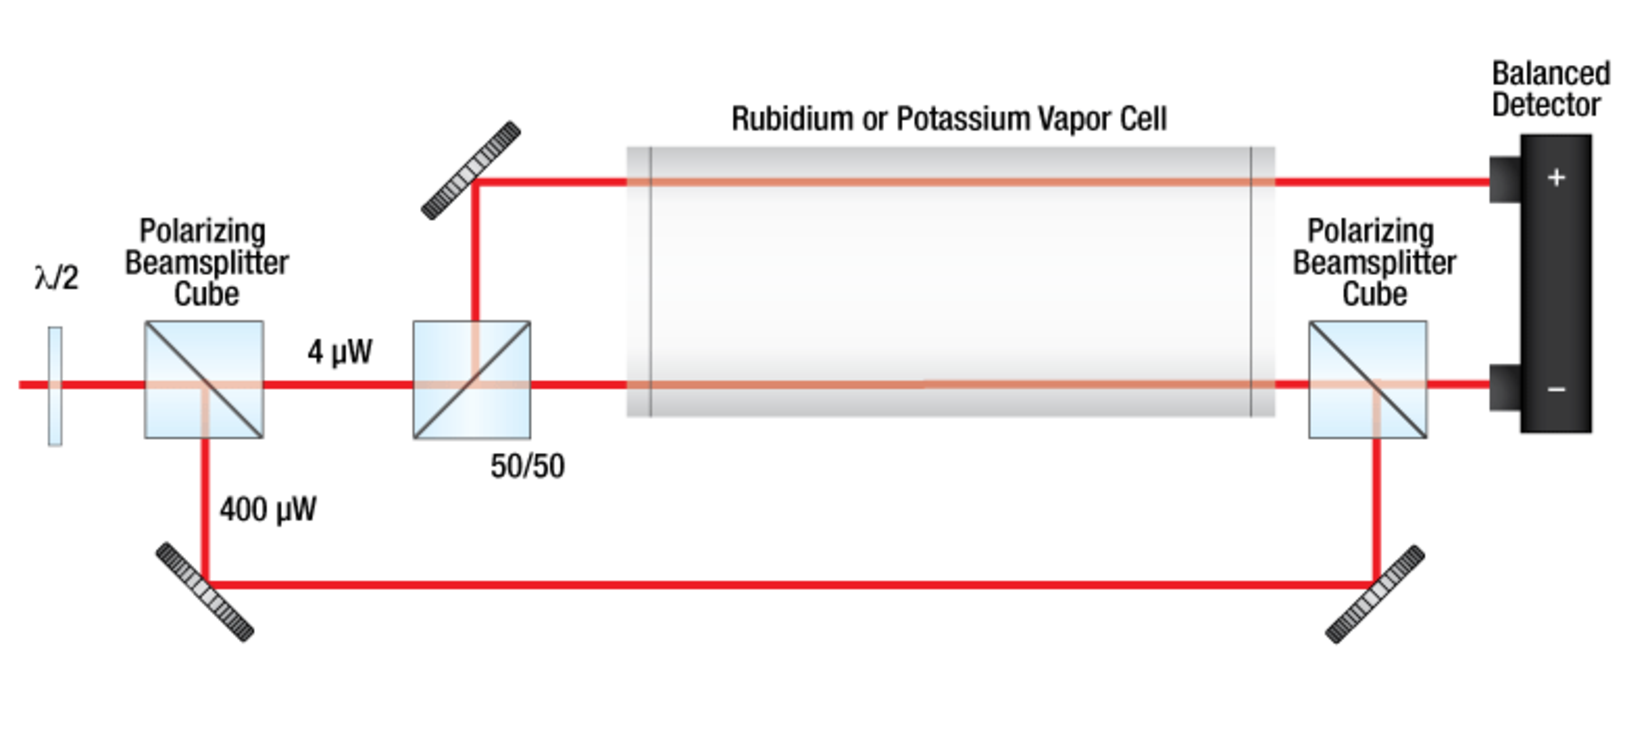
\includegraphics[width=6in]{SubDoppler.pdf}
\caption{Image from ThorLabs.~\cite{SubDoppler}}
\label{SubDoppler}
\end{figure}

Sub-Doppler begins with the laser passing through a half-wave plate to change the polarization of the light. Next the incoming laser beam is split using a polarizing beam splitter. The majority of the light is reflected around the rubidium cell, the light path at the bottom of Figure~\ref{SubDoppler}. The remaining light is passed through a fifty-fifty beam splitter, then both low power beams are passed through the rubidium cell. The uppermost low power beam in Figure~\ref{SubDoppler} will be used as a reference. The other low power beam, the beam in the center, passes left to right through the rubidium cell. The majority of the light, the high power beam, that was diverted around the rubidium cell is passed through the cell right to left in the center on top of the second low power beam. So the center beam in Figure~\ref{SubDoppler} is both a low power beam traveling left to right and a high power beam traveling right to left.

Inside the rubidium cell, atoms obey the Maxwell velocity distribution \textcolor{blue}{is this true?}. Atoms traveling 

The laser needs to be locked to the top of the fringe because that is the location which is known with precision. The difficulty with a top-of-fringe lock, different from a side lock, is that the intensity drops on both sides of the desired frequency and there is no way to tell which direction the frequency needs to be adjusted to match the peak frequency. To lock to the top of the fringe a lock-in method must be used. The lock-in output is the derivative of the input, so the input peak corresponds to an $x$ axis intercept on the output. The laser can easily be lock to the signal where it crosses zero.

In short, the laser light frequency, which is currently stabilized to both the etalon and reference cavity, is scanned by changing the length of the reference cavity.  When the reference cavity length matches the frequency of a the desired Rubidium hyperfine transition, the error signal will be fed back to the reference cavity.  This "locks" the reference cavity length so that the light transmitted through the cavity matches the transition frequency of that Rubidium line.  As usual, the reference cavity error signal still feeds back to the etalon to keep the band width of the laser at $50$ kHz. 
Setting up this stabilization was part of this thesis, but unfortunately the parts were back ordered.

\section{Laser Beam Intensity Profile}

The laser specifications state that the intensity profile is a two dimensional gaussian. So the intensity should be a gaussian in both $x$ and $y$ directions. 
\begin{equation}
\label{Gaussian}
I (x,y) = I_0\  e^{\frac{2 (x - x_0)}{w_x}} e^{\frac{2 (y - y_0)}{y_x}}
\end{equation}

In the above equation $I_0$ is the maximum intensity of the laser beam, $x_0$ and $y_0$ are the position offsets of the laser profile with respect to an arbitrary origin (see below), and $w_x$ and $w_y$ are the laser waists in the horizontal and vertical directions, respectively.  

We measure the intensity profile for two reasons.  The first is to confirm the spatial mode of the laser is in fact gaussian.  The second is to determine location of the minimum beam waists $w_{0x}$ and $w_{0y}$. 

The experimental procedure to measure the spatial profile is to use a straight edge (in our case a razor blade) mounted on a micrometer controlled translation stage.  The straight edge is then slowly more to transversely intersect the laser beam blocking more and more power as it goes.  A power meter is used to measure the laser beam power as the straight edge continually blocks more of the beam.  This procedure is done for both horizontal and vertical directions to extract both beam waists. The resulting graph of power versus position is the integral of the intensity profile because the change is power is measured for a small change in area. Therefore the experimental results should fit the integral of a gaussian,
\begin{equation}
\label{GaussianIntegral}
A\  Erf\bigg(\frac{\sqrt{2} ( x - x_0 )}{w}\bigg) + C
\end{equation}

Where $A$ is the amplitude, $C$ is a vertical offset, $x_0$ is a horizontal offset determined by our translation stage, $Erf$ denotes the error function and $w$ is the effective beam waist for the measured dimension at the that particular location on the $z$ axis (the direction of propagation). For a sample data set and fit using Equation~\ref{GaussianIntegral} see Figure~\ref{FitWaist}.

\begin{figure}[h!]
\centering
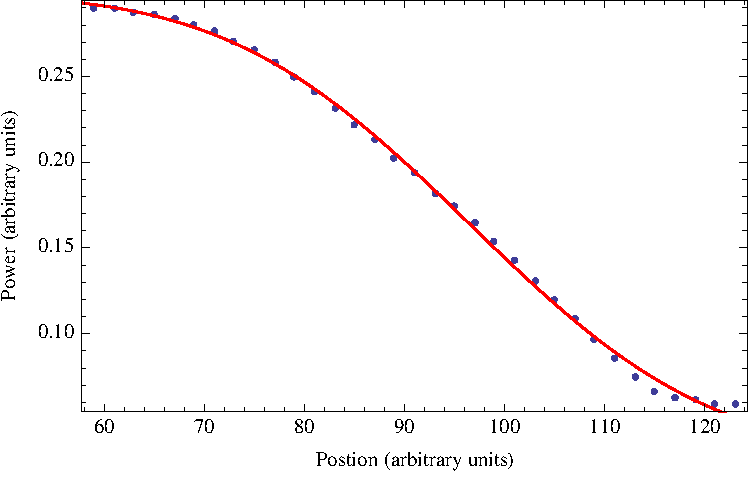
\includegraphics[width=6in]{FitWaist.pdf}
\caption{The blue data points are the power readings at various positions for the straight edge moving through the beam. The red fit is Equation~\ref{GaussianIntegral}.}
\label{FitWaist}
\end{figure}

Due to the uncertainty principle, all light fields diverge.  The smaller the initial waist of a laser beam, the quicker that beam diverges.  To measure the minimum laser waist in the longitudinal direction, we repeat the above measurement at a number of locations along the $z$ axis. Then the effective beam waist, with error given by the goodness of the fit, is plotted against the position on the $z$ axis. The measured minimum beam waist can be found by plotting the fitted waists for different positions on the $z$ axis.  These fitted waists can then be plotted and fitted using the theoretically expected divergence of beam waist to determine the size and location of the minimum beam waist. The theoretical divergence of the minimum beam waist is
\begin{equation}
\label{WaistDivergence}
w_0 \sqrt{1 + \frac{\lambda^2 \ (z-z_0)^2}{\pi \  w_0^2}}
\end{equation}

Where $w_0$ is the minimum beam waist in either the horizontal or vertical direction, $z_0$ is the location of the minimum beam waist along the $z$ axis and $\lambda$ is the wavelength of the light. $w_0$ and $z_0$ give us the characteristics of the laser beam in the desired transverse direction.  If the position of the minimum waist is different for the horizontal and vertical directions, we say that the beam is astigmatic.

Unfortunately the parts needed to produce $215$ nm were back ordered so we were unable to produce and characterize $215$ nm light used for the krypton experiment. However, we could produce the $235$ nm light used in the beryllium experiment. Since the laser set-up is identical for both experiments, except for the nonlinear crystals in the doubling cavities and the wavelength selected on the laptop for emission from the Ti:Sapphire, it was the $235$ nm light that we produced and characterized.

When we fully locked the Ti:Sapphire laser, the emitted beam was visibly diverging in the horizontal direction.  Even though we were wearing laser goggles, we can see the light diverging by letting the UV light hit a white card.  The white card fluoresces at many different wavelengths, some of which transmit through the goggles.   However, the above measurement suggested that our light was collimated, an obvious contradiction to our observations.  We realized that in addition to the $235$ nm light the laser also emitted $470$ nm light, a wavelength fully blocked by our laser goggles.  That blue light was interfering with our ability to measure the $235$ nm light.  We were measuring both wavelengths, not just the $235$ nm, and the blue light was close to collimated.

To avoid measuring the blue light with the power meter, we measured the beam diameter at various $z$ locations directly using a ruler with white paper taped to it. This was a rougher measurement, much more susceptible to systematic error due to parallax when measuring the diameter. However it was a relatively simple measurement that we could preform quickly and see the results were usable. The results we obtained are in Figures~\ref{WaistFit}. We found that the beam waist was $45 \pm 4$ cm before the mirror used to define the origin along the $z$ axis and that waist was $12.1 \pm 0.4 \mu$m with a divergence angle of $0.35 \pm 0.01^\circ$.

\begin{figure}
\centering
\begin{subfigure}{.5\textwidth}
  \centering
  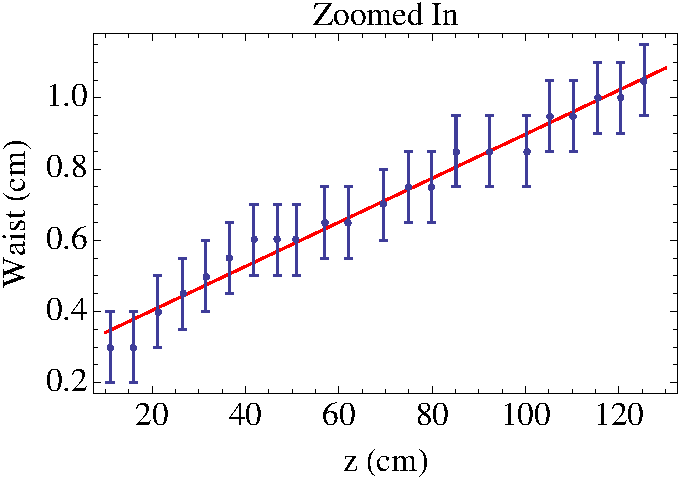
\includegraphics[width= .95\linewidth]{WaistFitS}
  \caption{Close-up results of waist measurements, showing error bars and goodness of fit.}
  \label{WaistFitS}
\end{subfigure}
\begin{subfigure}{.5\textwidth}
  \centering
  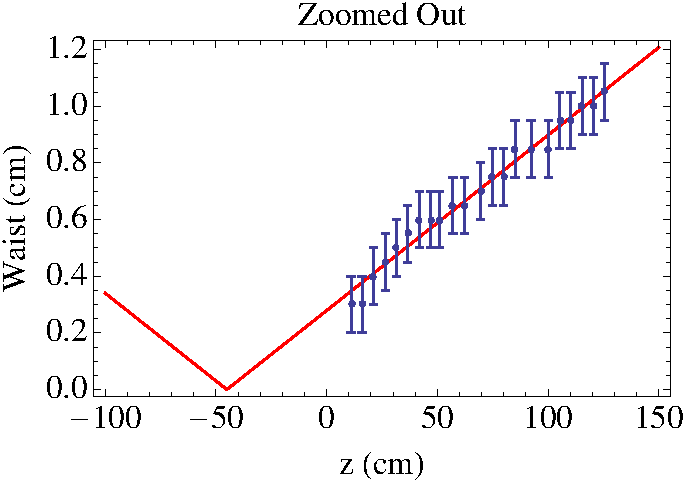
\includegraphics[width= .95\linewidth]{WaistFitL}
  \caption{The projection of the fit showing location of the beam waist.}
  \label{WaistFitL}
\end{subfigure}
\caption{The data from measuring the twice the effective beam waist with a fit using Equation~\ref{WaistDivergence}. The location of the beam waist is $-45 \pm 4$ cm, that is $45$ cm before the location defined as the origin. And the waist is $12.1 \pm 0.4 \mu$m with a divergence angle of $0.35 \pm 0.01^\circ$.}
\label{WaistFit}
\end{figure}

Based on these results, we decided to use a $200$ mm cylindrical lens which should give us a beam waist of $\approx 3$ mm along the horizontal axis. When we measured the light after installing the lens we got a beam waist of $3.5 \pm .8$ mm which agrees within uncertainty with our expected value for the beam waist. The laser was very close to collimated, our method of beam waist measurement was not precise enough to measure any divergence.


\section{Conclusion}


\section{Appendix}

\textcolor{magenta}{Put Mathematica notebooks here!}

\singlespacing{
\begin{thebibliography}{18}

\bibitem{UndergroundWater} N. C. Sturchio, X. Du, R. Purtschert, B. E. Lehmann, M. Sultan, L. J. Patterson, Z.-T. Lu, P. Mueller, K. Bailey, T. P. O'Connor, L. Young, R. Lorenzo, B. M. Kennedy, M. van Soest, Z. El Alfy, B. El Kaliouby, Y. Dawood, and A. M. A. Abdallah, ``One million year old groundwater in the Sahara revealed by krypton-81 and chlorine-36'', Geophysical Research Letters 31(5), L05503 (2004)

\bibitem{Nuclear1} M. B. Kalinowski, H. Sartorius, S. Uhl, W. Weiss, ``Conclusions on plutonium separation fromatmospheric krypton-85 measured at various distances from the Karlsruhe reprocessing plant,''
Journal of Environmental Radioactivity 73 (2), 203e222 (2004)

\bibitem{Nuclear2} R. S. Kemp, C. Schlosser, ``A performance estimate for the detection of unde- clared nuclearfuel reprocessing by atmospheric 85Kr,'' Journal of Environmental Radioactivity 99, 1341e1348,
2008 Erratum Journal of Environmental Radioactivity 100, 99 (2009)

\bibitem{ANL} C. Y. Chen, Y. M. Li, K. Bailey, T. P. O'Conner, L. Young, and Z.-T. Lu, ``Ultrasensitive isotope trace analyses with a magneto-optical trap,'' Science 286, 1139. (1999)

\bibitem{EBeam1} R. S. Freund, ``High current low voltage electron bombarder for excitation of a molecular beam,'' Rev. Sci. Instrum. 41, 1213 (1970)

\bibitem{EBeam2} R. D. Rundel, F. B. Dunning, and R.F.Stebbings, ``Velocity distributions in metastable atom beams produced by coaxial electron-impact,'' Rev. Sci. Instrum. 45, 116 (1974)

\bibitem{EBeam3} B. Brutschy and H. Haberland, ``High-intensity beam of metastable helium-atoms with good velocity resolution,'' J. Phys. E 10, 90 (1977)

\bibitem{EBeam4} T. W. Riddle, M. Onellion, F. B. Dunning, and G. K. Walters, ``Polarized he (23s) thermal metastable atom source,'' Rev. Sci. Instrum. 52, 797 (1981)

\bibitem{Plasma1} M. E. Bannister and J. L. Cecchi, ``Metastable argon beam source using a surface-wave sustained plasma,'' J. Vac. Sci. Technol. A 12, 106 (1994)

\bibitem{DCDis1} D. W. Fahey, W. F. Parks, and L. D. Schearer, ``High-flux beam source of thermal rare-gas metastable atoms,'' J. Phys. E. 13, 381 (1980)

\bibitem{DCDis2} M. J. Verheijen, H. C. Beijerinck, L. H. A. M. v. Moll, J. Driessen, and N. F. Verster, ``A discharge excited supersonic source of metastable rare-gas atoms,'' J. Phys. E 17, 904 (1984)

\bibitem{DCDis3} J. A. Brand, J. E. Furst, T. J. Gay, and L. D. Schearer, ``Production of a high-density stateselected metastable neon beam,'' Rev. Sci. Instrum. 63, 163 (1992)

\bibitem{DCDis4} J. Kawanaka, M. Hagiuda, K. Shimizu, F. Shimizu, and H.Takuma, ``Generation of an intense low-velocity metastable-neon atomic-beam,'' Appl. Phys. B 56, 21 (1993)

\bibitem{DCDis5} W. Rooijakkers, W. Hogervorst, and W. Vassen, ``An intense collimated beam of metastable helium atoms by two-dimensional laser cooling,'' Opt. Commun. 123, 321 (1996)

\bibitem{RFDis1} O. Carnal and J. Mlynek, ``Youngs double-slit experiment with atoms - a simple atom interferometer,'' Phys. Rev. Lett. 66, 2689 (1991)
 
\bibitem{RFDis2} C. Y. Chen, K. Bailey, Y. M. Li, T. P. O'Connor, Z.-T. Lu, X. Du, L. Young, and G. Winkler, ``Beam of metastable krypton atoms extracted from a rf-driven discharge,'' Rev. Sci. Instrum. 72, 271 (2001)

\bibitem{FirstExcited} V. Kaufman, ?Wavelengths and energy-levels of neutral kr-84 and level shifts in all kr even isotopes,? J. Res. Natl. Inst. Stand. Tech. 98, 717 (1993)

\bibitem{NIST} A. Kramida, Yu. Ralchenko, J. Reader, J. and NIST ASD Team (2013). NIST Atomic Spectra Database (version 5.1), [Online]. Available: \url{<http://physics.nist.gov/asd>} [Wednesday, 15-Jan-201422:06:55 EST]. National Institute of Standards and Technology, Gaithersburg, MD.

\bibitem{KrTransitions} W. E. Ernst and E. Schulz-Gulde, ``Transition probabilities for Kr I lines from wall-stabilized arc measurements,'' Physica B+C 93, 136–144 (1978)

\bibitem{Cannon} B. D. Cannon, ``Model calculations of continuous-wave laser ionization of krypton,'' PNNL-12253 (1999)

\bibitem{Ti:S} M Squared Lasers Ltd, ``SolsTiS - Narrow Lindwidth, Tunable CW Ti:Sapphire Laser User Manual'' v10.3

\bibitem{ECDX} M Squared Lasers Ltd, ``ECD-X - Ultra-compact Frequency Doubling Accessory User Manual'' v1.8

\bibitem{SubDoppler} ThorLabs, Saturated Absorption Spectroscopy Systems \url{<http://www.thorlabs.com/newgrouppage9.cfm?objectgroup_id=5616>}


\end{thebibliography}
}

\end{document}